\section{Knowledge and economic growth. A history of discovery,
invention and innovation.}

\subsection{On the nature of economic growth}

\paragraph{How to measure economic growth}

Basics:
\begin{itemize}
    \item The output of an economy, in a specific counry, over a certain period,
        is measured in terms of GDP - Gross Domestic Product.
    \item GDP gives the monetary value of final goods and services - that
        are those bought by the final user (net of intermediate consumption)
    \item The simplest measure of economic growth is the annual increase
        of GDP.
    \item But it is better to correct for changes in inflation and population
        and use the annual increase of real GDP per capita as a proxy for
        economic growth.
\end{itemize}
GDP is a very crude measuere: It only counts transactions that can be given a
monetary value. Here are a few examples of what is excluded from GDP:
\begin{itemize}
    \item Unpaid houshold or voluntary work (on the positive side)
    \item So-called externalities like environmental destruction and
        pollution (on the negative side).
    \item Free digital goods like online search engines and new digital
        commons like Wikipedia or social media.
\end{itemize}

GDP is a short-term measure:
It only considers monetary transactions and flows and as such totally ignores
capital assets of all kinds such as the depletion of resources or loss of
biodiversity, nor does it account for the improvement, decay, or even destruction
of infrastructure or the value of human and social capital.

For example, the destruction of assets in wartime will not show up in GDP,
but the 'consumption' of weaponry and the reconstruction after the war will
boost GDP growth.

\paragraph{Economists understand little about the causes of growth}

\begin{itemize}
    \item growth is a consequence of capital accumulation (Solow,Swan,\dots)
    \item availability of land and resources\dots (taken for granted in a class
        of economic models)
    \item growth as a consequences of (Cobbs-Douglas) relations between labor,
        capital and technology; endogenous growth theories (Roman, Kramers\dots)
    \item growth made possible by legal and enforced framework (property rights)
    \item cultural and financial incentives for private efforts and innovations
    \item role of government, quality of governance and trust
    \item anti-corruption\dots
\end{itemize}

\paragraph{Exponential growth in the aggregate, with a rich underlying
dynamical process}

Using modern data analysis techniques, Lera and Sornette proved that economic
growth is bimodal:
\begin{itemize}
    \item With one regime of expansion with strong growth, and another regime
        of consolidation with low growth or decline.
    \item The system naturally switches between these two regimes in one single
        dynamical process.
    \item In this view, growth and consolidation are two sides of the same coin.
\end{itemize}

\paragraph{Secular bopolar growth rate of the real US GDP per capita.}
A long term average growth rate of real GDP per capita of 2\% per year is
obtained by regime shifts between regimes of high growth ($\sim 3\%$ per year)
and regimes of low growth ($<1\%$ per year).

Structural characteristics of growth: regime shifts and bimodal patterns

\subparagraph{Lesson 1:} Growth occurs in cycles and there is persistent
hubris in extrapolating the high-growth regimes

\vspace{1\baselineskip}

It is important to realize that:
\begin{itemize}
    \item The strong-growth modus is seen at the norm and the healthy state of
        economy, and the low-growth as an aberratoin and a symptom of disease
        that needs to be cured.
    \item Therefore, we always extrapolate the high-growth regimes.
    \item However, growth is a single bimodal process of overshooting during
        boom followed by correction and consolidation.
    \item The correction is as much part of the process as the boom.
\end{itemize}

To explain where the coarse-grained long-term exponential growth comes from,
we must first make a distinction between things and ideas, rival and nonrival
goods.

\paragraph{Things versus ideas}

Things (objects, goods) are rival:
\begin{itemize}
    \item As more people drive on a highway or use water for irrigation, there
        are fewer of these goods to go around\dots
    \item To increase the productivity of each person in an economic system using
        things (like a computer), you need to give each person such a thing.
        Economic output per capita, under such conditions, is proportional to
        the capital per person.
    \item in a closed economy, capital is subject to diminishing returns:
        'The first barrel of fertilizer does wonders for a plot of land; the
        tenth only burns the crop.'
    \item This leads to a kind of steady-state, end-of-growth, unless exogenously
        something happens (e.g. technological change)
\end{itemize}
Ideas, in contrast, are nonrival:
\begin{itemize}
    \item As more and more people use the Pythagorean theorem of the Java
        programming language, there is not less and less of the idea to go
        around.
    \item Ideas are not depleted by use, and it is technologically feasible
        for any number of people to use an idea simultaneously once it has
        been invented.
    \item You can increase the productivity of any number of people in an
        economic setting by inventing a single new idea. Economic output per
        capita, under such conditions, is proportional to the total stock of
        ideas. Taking logs and derivatives, the economic growth is proportional
        to the growth rate of the total stock of ideas.
\end{itemize}

\begin{figure}[h]
    \centering
    \begin{subfigure}{0.48\textwidth}
        \centering
        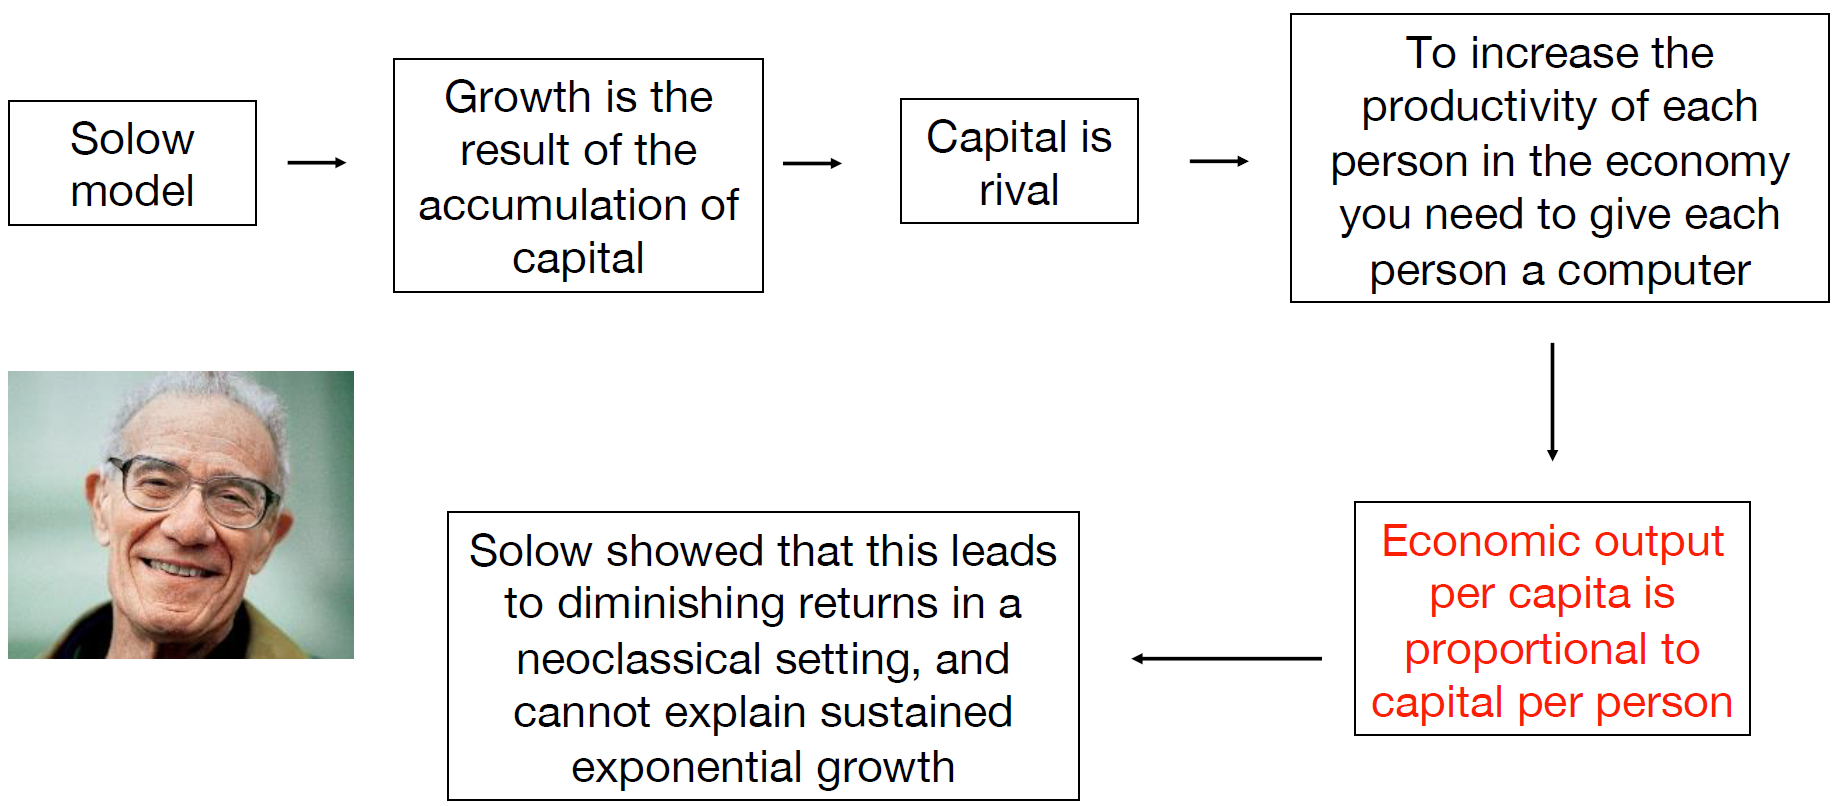
\includegraphics[width=\textwidth]{Pictures/Solow.png}
        \caption{Sollow Model}
    \end{subfigure}
    \hspace{5pt}
    \begin{subfigure}{0.48\textwidth}
        \centering
        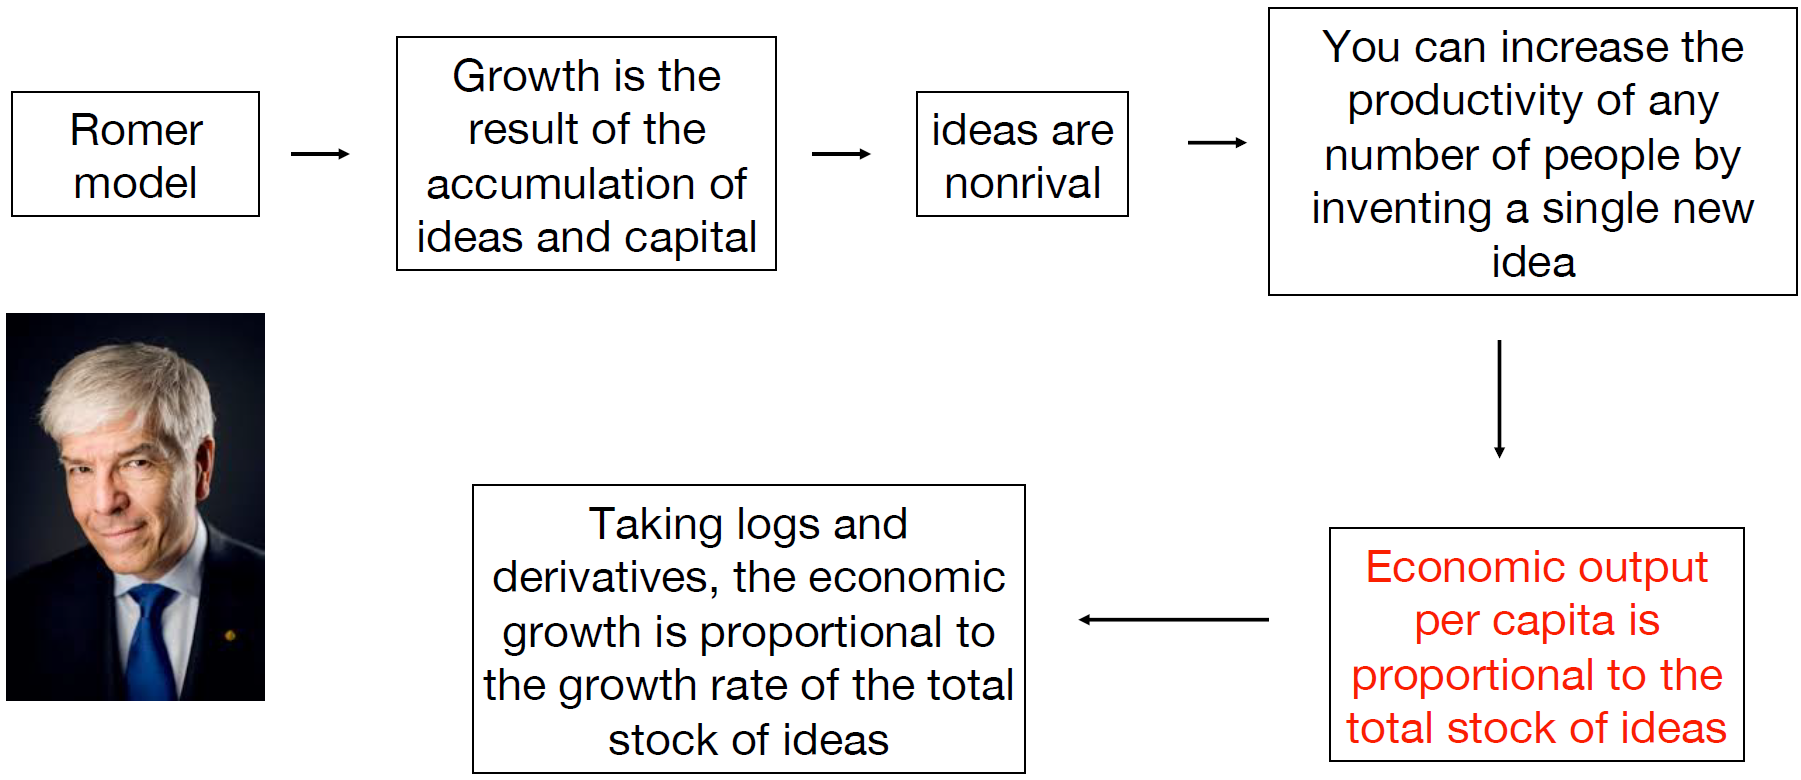
\includegraphics[width=\textwidth]{Pictures/Romer.png}
        \caption{Romer Model}
    \end{subfigure}
\end{figure}

\paragraph{Endogenous growth theory}

\begin{itemize}
    \item Economic growth is proportional to the growth rate of the overall
        stock of ideas.
    \item The overall stock of ideas grows with the increase of resources
        allocated to finding new ideas (people, capital,\dots)
    \item But it plateaus when ideas become harder to find (S-curve, logistical
        process\dots)
    \item The economy can only grow at a constant rate over the long run if
        research productivity (output/input, or results/investment) is
        constant.
\end{itemize}

In the following parts, we will zoom in on the following three questions:
\begin{itemize}
    \item Are ideas harder to find?
    \item What exactly is 'knowledge'?
    \item Is there a constant rate of knowledge accumulation?
\end{itemize}

\subsection{On the productivity of research}

Discussing question 1: 'Are ideas harder to find?'

\vspace{1\baselineskip}

Despite vast increase in in the time and money spent on research, progress
is barely keeping up with the past. What went wrong?

\vspace{1\baselineskip}

Number of PhD students increase and more is invested in research. On the surface,
this is encouraging. But for all this increase in effort, are we getting a proportional
increase in our scientific understanding? Or are we investing vastly more
merely to sustain (or even decline in) the rate of scientific progress?

\vspace{1\baselineskip}

Economic growth (e.g. 2\% or 5\%) = Research productivity (falling) $\times$
Number of researchers (rising)

\vspace{1\baselineskip}

To have a constant research productivity, the effective number of researchers
and the US TFP growth should behave similarly. It turns out that we need more
than $20 \times$ more research capacity (input), to sustain a declining
productivity (output).

\vspace{1\baselineskip}

\paragraph{Are ideas getting harder to find?}

In a paper in the American Economic Review, Bloom et al. give some compelling
evidence:
\begin{itemize}
    \item Moore's law: 'the number of researchers required to double chip density
        today is more than 18 times larger than the number required in the early
        1970s\dots Research productivity in this case is declining sharply, at
        a rate of 7\% per year.'
    \item Research productivity for crop seed yields and mortality improvements
        associated with cancer and heart diseases declines at a rate of 5\% per
        year.
    \item Looking at firm-level data, research productivity declines at a rate
        of 8-10\% per year dependent on the data source.
\end{itemize}

\paragraph{But continuous increase in R\&D investment}

Over the past 70 years, the non-financial business debt in the U.S., as a
fraction of GDP has increased from 40\% to 140\%. However, the contribution
of investments to GDP has hovered between 15\% and 20\%.

Where has the increasing debt of American businesses been used for, if not
for CAPEX and fixed assets?

The most probable answer is that this debt is used to finance goodwill
(e.g. from M\&A activity) and intangible assets (R\&D, patents,\dots)

\subsection{On the nature of knowledge}

Discussing question 2: 'What exactly is knowledge?'

\subsubsection{What is "knowledge"?}

What is the difference between discovery, invention and innovation?

\paragraph{Discovery}

The first-time recognition of something already existing:
\begin{itemize}
    \item \underline{A thing}: a new mine or an oil well, a continent, an
        island, a moon, planet, star, a fundamental particle (such as the
        electron or a neutrino)\dots
    \item \underline{An idea}: an insight, like the discovery of a fundamental
        law of nature.
\end{itemize}

The result of a process of exploration:
\begin{itemize}
    \item A high-risk endeavor into the unknown
    \item Willingness to employ substantial expenses without any certainty
        for future results or returns.
\end{itemize}

To use the words of the opening lyrics of the Star Trek television series,
discovery is 'to boldly go where no man has gone before'.

\subparagraph{The challenges of exploration}
According to Herbert Simon exploration requires:
\begin{itemize}
    \item tolerance of ambiguity
    \item patience: learning-by-doing, accumulation of knowledge, trial-and-error
    \item luck / serendipity
    \item persistence / dilligence
    \item 'intuition': use of smart heuristics
\end{itemize}

It is a high risk endeavor, where the payoff is almost impossible to estimate.

\paragraph{Invention}

The creation of something new:
\begin{itemize}
    \item \underline{A thing}: a mechanical machine like a steam engine, a
        scientific instrument like a microscope
    \item \underline{An idea}: a mathematical algorithm, like artificial
        intelligence, or chemical process like the Haber-Bosch ammonia
        synthesis to produce fertilizers, or the Bessemer process to decarbonize
        iron in the production of steel.
\end{itemize}

The result of a creative process:
\begin{itemize}
    \item Engineering
    \item often combined with stubborn trial-and-error tinkering
    \item and a large dose of luck
\end{itemize}

\paragraph{Innovation}

Combining existing things and ideas in a novel way to:
\begin{itemize}
    \item Solve a problem,
    \item optimize a process
    \item or bring a new products or service to the market.
\end{itemize}

The result of a process of exploitation:
\begin{itemize}
    \item Taking advantage, by doing combinatorics, of prior creative inventions
        and explorative discoveries
    \item Low (or at least known) risk endeavor into charted territory
    \item where one can make a decent estimation of the prospect of success
\end{itemize}

\subsection{How do we innovate, invent or discover?}

How to understand the incentives?

\paragraph{The whole is greater than the sum of its parts}

$R \sim c^\beta$ where the production $R$ is defined as the total number
of commits measured per 5-day time window for the Apache Web server and
$c$ is the number of active contributors in the same 5-day time window.
$\beta$ decreases with increasing number of developers.

\vspace{1\baselineskip}

Six design principles to help managers deal with the challenge of
Productive/Creative Bursts.
\begin{enumerate}[1)]
    \item transparency
    \item bottom-up incentives and self-censored clans
    \item emergent technology
    \item problem front-loading
    \item distributed screening
    \item Modularity
\end{enumerate}

\paragraph{The skill-success gap}

Mechanisms of Luck
\begin{itemize}
    \item Gibrat's law, proportional growth, and the Matthew effect
    \item Winner-takes-all
    \item Adverse selection
    \item Male-male competition and evolution
    \item Big statistic replication crisis
    \item Hyped big data, artificial intelligence, and machine learning
\end{itemize}

\paragraph{Skill versus luck}
\begin{align*}
    \frac{d S_t}{S_t} = \mu dt + \sigma d W_t
    \hspace{10pt} , \hspace{10pt}
    \ln(S_t) \sim \klammer{\mu - \frac{\sigma^2}{2}} T + x_i \sigma \sqrt{T}
\end{align*}
\begin{itemize}
    \item $S$, the size of a firm
    \item $\mu$, the growth rate
    \item $W$, Wiener process, stochaistic random noise
    \item $\sigma$, volatility
    \item $\mu_{skill}$, the mean of the skills of the $N$ agents
    \item $\sigma_{skill}$, the standard deviation of the skills of the $N$ agents
    \item $\mu_{luck}$, the mean of the luck of the $N$ agents
    \item $\sigma_{luck}$, the standard deviation of the luck of the $N$ agents. 
\end{itemize}
There is a characteristic time $T^\ast$ at which skill and luck will contribute
equal the outcome of the GBM process. At that time $T^\ast$ satisfies $\mu T^\ast
= \sigma \sqrt{T}$, yield $T^\ast = \klammer{\frac{\sigma}{\mu}}^2$.

\vspace{1\baselineskip}

Sharpe ratio - see lecture slides 26.05\footnote{\url{https://xyotta.com/cfiles/1236}}

\subsection{The industrial revolutions, four waves of industrial innovation}

Is there a constant rate of knowledge accumulation?

\begin{enumerate}[]
    \item \underline{Industry 1.0}: The Industrial Revolution begins.
        Mechanization of manufacturing with the introduction of steam and
        water power.
    \item \underline{Industry 2.0}: Mass production assembly lines using
        electrical power.
    \item \underline{Industry 3.0}: Automated production using electronics,
        programmable logic controllers (PLC), IT systems and robotics
    \item \underline{Industry 4.0}: The 'Smart Factory'. Autonomous decision
        making of cyber physical systems using machine learning and Big Data
        analysis. Interoperability through loT and cloud technology.
\end{enumerate}

\paragraph{Industry 1.0} The industrial revolution (1760-1840)

Technology:
\begin{itemize}
    \item Mechanization of manufacturing with the introduction of machine tools
        and steam power
    \item Mainly focused around the textile industry (cotton, wool, silk) e.g.
        spinning jenny
\end{itemize}
Energy:
\begin{itemize}
    \item Beginning of the use of coal to power steam engines (steam power),
        in addition to muscular power (animals and humans) and traditional
        biofuels.
\end{itemize}
Geography:
\begin{itemize}
    \item Originally started in the UK
\end{itemize}
Infrastructure:
\begin{itemize}
    \item Networks of canals and improved waterways
    \item Paved 'macadamized' roads (John McAdam)
    \item First introduction of railroads in the UK (ending in the Railway
        Mania of the 1840s)
\end{itemize}

\paragraph{Industry 2.0} The technological revolution (1870-1910)

Technology:
\begin{itemize}
    \item Electricity: steam turbine, generator, transformer, engine, incandescent
        bulb, light
    \item Steel (Bessemer process)
    \item Combustion engine
    \item Chemistry: synthesis of new materials and chemical products
\end{itemize}
Management:
\begin{itemize}
    \item Economy of scale: It is cheaper to manufacture products in large quantities
    \item Vertical integration of the supply chain from raw materials (e.g. iron
        ore and coal) to final product (e.g. steel railway track)
    \item Scientific management (Taylorism): new empirical organization methods
        to improve efficiency and labor productivity in large scale businesses
        that operate over vast areas.
\end{itemize}
Geography:
\begin{itemize}
    \item US, UK, Continental Europe
\end{itemize}
Energy:
\begin{itemize}
    \item Coal and the birth of the high energy society
\end{itemize}
Infrastructure:
\begin{itemize}
    \item Networked house (electricity, sewage, streaming water, telephone,
        central heating, etc)
    \item Electrified underground railways (Paris Métro, London Tube, Berlin U-Bahn,\dots)
    \item Linking of existing railway networks to allow for long-distance
        travelling (e.g. Paris-Istanbul with orient express, Moscow-Vladivostok
        with Trans-Siberian Railway,\dots)
    \item Transatlantic telegraph cable
    \item Transcontinental steamhip routes
    \item Sea canals (Suez, Panama)
    \item City planning
\end{itemize}

\vspace{1\baselineskip}

\begin{itemize}
    \item New structural forms with the application of new engineering techniques and
        materials such as glass and steel.
    \item The rise of the modern city: straight boulevards, buildings with equal
        hights, parks and squares, new sewer systems, infrastructure for fresh
        drinking water\dots
\end{itemize}

\paragraph{Industry 3.0} The electronic revolution (1947-20xx)

Technology:
\begin{itemize}
    \item PLC (Programmable Logic controllers)
    \item Computers (transistor, Integrated circuits, computer chips, microchips)
    \item Software and computer programs, user interfaces
    \item Robotics
    \item Mobile phones / smartphones
\end{itemize}
Infrastructure
\begin{itemize}
    \item Automobile: Interstate highway systems
    \item Aircraft: Jet Age (aircraft powered by turbine engines),
        Long-distance commercial flights
    \item Digital: internet, worldwide web
    \item Mobile
\end{itemize}
Energy
\begin{itemize}
    \item Oil and gas
    \item Nuclear
\end{itemize}

\begin{enumerate}[]
    \item \underline{Phase 1}: Mainframe computers connected through ARPANET
        (US department of defense) in TCP/IP protocol $\rightarrow$ internet
        mainframe
    \item \underline{Phase 2}: Desktop, laptop, tablets and smartphones connected
        in WWW (HTMP - HyperText Markup Languate, invented in CERN) $\rightarrow$
        internet of people, data and services
\end{enumerate}

\paragraph{Industry 4.0} The cyber revolution (20xx - \dots)

Phase 3: Cyber Physical Systems $\rightarrow$ internet of everything

\vspace{1\baselineskip}

People to people, people to machines and machines to machines

\vspace{1\baselineskip}

Technology: Cyber physical systems: physical and software components are
deeply interwined
\begin{itemize}
    \item Machine to machine technology
    \item Smart: Things measure, analyse and act autonomously
    \item Self-organization of technology, machines, human beings\dots
    \item internet of things
    \item Sensors
    \item Artificial intelligense, algorithms, big data analysis
    \item Augmented reality
    \item Additive manufacturing
    \item Cloud computing
\end{itemize}

\subsection{A critical assessment of the industry 1.0 : 4.0 framework - The
Chinese case}

\begin{itemize}
    \item It is very much Western-centric and describes technological progress
        as a continuous and steady process, from industry 1.0 up to industry
        4.0, like the different deployments of a software package.
    \item In reality, progress (in technology, economy, society,\dots) is
        discontinuous and punctuated
\end{itemize}

\paragraph{Han Dynasty in China} (207 BCE - 9 CE) The achievements of the Han
dynasty in the field of science and technology were concentrated in hydroproject,
architecture, mathematics, calendars and other technological fields, Han dynasty
witnessed some of the most significant advancements in premodern Chinese science
and technology. 'The consatenation of Han advances laid strong technical foundations
for the development of the world's most persistent empire - which was, until the
18th century also the world's richest economy\dots'

\paragraph{Boreholes and mining shafts} (206 BC - 220 AD)
Borehole drilling has a long history. By at least the Han Dynasty, the
Chinese used deep borehole drilling for mining and other projects. The Chinese
method of deep drilling was accomplished by a team of men jumping on and off
a beam to impact the drilling bit while the boring tool was rotated by buffalo
and oxen. By the first century BC, Chinese craftsmen cast iron drill bits and
drillers were able to drill boreholes up to 1500 m deep. It wasn't up until
the 19th century that Europe and the West would catch up and rical ancient
Chinese borehole drilling technology.

\paragraph{Hydraulics} (206 BC - 220 AD)
By the Han Dynasty, the Chinese developed various uses for the waterwheel. In
his Balanced Discourse, the philosopher Wang Chong first described the square-pallet
chain pump that could pump water and other substances. Their primary use was for
lifting water into irrigation ditches, but chain pumps were also used in public
works programs, such as when Zhang Rang used them to lift water into pipes.
The water was used to provide the capital Louyang with clean water. In 31 AD
Du Shi is credited with being the first to apply hydraulic power to operate bellows
(air-blowing device) in metallurgy. This is a great invention in ancient China
and the history of mechanical engineering, about a thousand years earlier
than Europe.

\paragraph{The Seismograph} (132 BC)
The Han court was responsible for the major efforts of disaster relief when natural
disasters such as earthquakes devastated the lives of commoners. Zhang Heng, an
early Chinese scientist, created the first device for detecting distant earthquakes
had occured in a location indicated by a specific cardinal or ordinal direction,
which he introduced in the Han court in 132 AD. Its design was simple - an urn
equipped with a pendulum. When it picked up a vibration, it dropped a ball from
the mouth of a metal dragon into a metal frog, creating a loud clang. The first
time that happened, nobody in the court reportedly felt anything, but a few
days later, a messenger from a villate 400 miles away arrived to inform the
emperor that an earthquake hat occured there.

\paragraph{The Wheelbarro} (100 BC)
The Wheelbarrow was developed in China perhaps as early as 100 BC. It can
acconodate a much larger wheel, thus reducing the rolling resistance, and by
having the wheel almost directly under the load it reduced the weight on the
user's arms.

\paragraph{The Invention of Paper} (105 AD)
Cai Lun, an eunuch in the Han court in 105 AD, is credited as the inventor of
the first really high-quality writing paper, which he fashioned by crushing
and combining tree bark, hemp, linen rags, and scraps from fishing nets and
then treating the mixture with lye to break it down into finer fibers.

\paragraph{Longshou Canal} (120-111 AD)
The Longshou Canal was built in 120 BC - 111 BC during the Han Dynasty, which
is the first underground canal in China's history with more than 5 km, the
Longshou Canal making use of the shaft-tunnel method. Its completion allowed
irrigation of more than 40,000 hectares of saline land and increased the yield
of its farmland by more than 10 times. This hydoproject method spread to Central
and Southwest Asia through the Silk Road. The Longshou canal has provided
valueble experience for the world's water conservancy industry.

\paragraph{Gunpowder weapons in the Song dynasty} (969-1044 AD)
The earliest-known existent written formulas for gunpowder come from the
Wujing Zongyao text of 1044, which described explosive bombs hurled from
catapults. The earliest developments of the gun barrel and the projectile-fire
cannon were found in late Song China. These 'fire-lances' were widespread in
use by the early 12th century, featuring hollowed bamboo poles as tubes to
fire sand particles (to blind and choke), lead pellets, bits of sharp metal
and pottery shards, and finally large gunpowder-propelled arrows and rocket
weaponry.

\paragraph{Hydraulic-powered astronomical clock tower}
Created by Su Song of the Song Dynasty in 1088 AD, it has three functions of
observing the movement of the celestial bodies, demonstrating the changes in
the sky, and accurately telling the time. It is the oldest astronomical clock
in the world, representing the wisdom of polymaths and mechanical engineering
of the Song Dynasty.

\paragraph{Jiaozi - The first paper money in history} (1023 AD)
Jiaozi, the earliest paper money used in the world, first appeared in the
Sichuan region and was issued in Chengdu in 1023. In the beginning, the Jiaozi
was actually a certificate of deposit, with the development of the market economy,
the use of Jiaozi became more and more widespread, and in a short time it turned
from a commercial credit certificate into an official legal currency with all the
basic elements of modern paper money. Compare with western, the first
government-issued paper money in the western world was in the late 17th century,
more than 600 years after China.

\subsection{A critical assessment of the industry 1.0 : 4.0 framework}

Are the 4 different periods equal? Do they represent the same amount of "progress"?
Maybe some inventions are more important than others?

\vspace{1\baselineskip}

Clean water and better hygene lowered the death rate extremely. Older inventions
such as amnesthetics is much more important than for example VR gogglles for
user experience. New inventions replaced older ones. Fake news are nothing
new.

\subsection{Conclusion}

We discussed the followign three fundamental questions.
\begin{itemize}
    \item Are ideas harder to find? Yes
    \item What is the meaning of knowledge? Semantics do matter, knowledge
        itself has a fine-grained structure and should be disentangled into
        discovery, invention and innovation.
    \item Is there a constant rate of knowledge accumulation? No, it follows
        a complex process with ruptures, paradigm shifts, revolutions
\end{itemize}
It seems that the puzzle of economic growth has not been solved completely yet.
And maybe a next step forward could be found through a better understanding
of the structure and the dynamics of the knowledge accumulation process.

\subsection{In our research group, we are trying to contribute to solving this
puzzle. Here are some very recent results}

\paragraph{Is there a constant rate of knowledge accumulation?}
\begin{itemize}
    \item We assembled a prioritary dataset of great inventors and discoverers
        over the past two milennia.
    \item You can see peeks in the graph during the industrial revolutions
\end{itemize}

\paragraph{Knowledge is not homogeneously distributed in space or time and across
scientific disciplines}

\begin{itemize}
    \item In time, a rich pattern of waves can be observed coinciding with industrial
        and technological revolutions and scientific paradigm shifts.
    \item In space, we see that the UK has been the major participant in the three
        industrial revolutions from the past 250 years, in the first half of that
        period, the European Continent was its main challenger; in the second
        half it was the US. It is eye-opening to see that European Continent's
        steady decline since the 1900s, except perhaps in biology, medicine
        and genetics.
    \item Across scientific disciplines, we see a general superiority in physics,
        mathematics and astronomy, a long-term decline in Chemistry, and a strong
        increase in biology, medicine in genetics between 1910 and 1970.
\end{itemize}
Since 1970 all disciplines are in decline across all geographical regions. Our
data would suggest that industry 4.0 is fully driven by innovation, and that
the rate of discovery and invention is in a secular decline. Could this be one
of the fundamental drivers behind dynamics of the Fool's Gold Age?

\subsection{How to quantitatively formulate the problem of exploitation of an
existing set of invention,innovation and exploration}

\paragraph{What is the investment universe?}

\begin{itemize}
    \item The vast majority of papers on portfolio selection starts with a
        sentence of the form 'The investment universe consists of one risk-free
        and $N$ risky assets'.
    \item In practice, even if $N$ is large, it is arguably not the case that
        the $N+1$ assets present in the specified investment universe cover
        every conceivable investment opportunitiy for the agent. Large investors
        are continuously looking for new investment opportunities (private
        investment, start-ups, crypto-assets, etc)
    \item Rather, these are the investment opportunities which are salient
        to the agent and well understood in terms of their relevant distributional
        properties.
\end{itemize}

\paragraph{Exploration of new investment opportunities}
\begin{itemize}
    \item We propose an extension of the classical setting with a fixed
        investment universe by giving the agent the option to explore for new
        investment opportunities.
    \item If this option is exercised, the agent chooses to devote a part of
        his/her wealth for exploration.
    \item Exploration results in the discovery of a new asset, whose distribution
        properties depend on the amount devoted to exploration in a way that the
        asset becomes more attractive to the agent when a larger amount is devoted
        to exploration.
    \item After discovery of the new asset, the agent of the extended investment
        universe in order to optimize her preferences over the resulting
        terminal wealth.
    \item trade-off between exploration and exploitation
\end{itemize}
\paragraph{Investment setting}
\begin{itemize}
    \item We consider a single-period model of an agent with mean-variance
        preferences.
    \item Classical model: dixed investment universe $\mathcal{U}$ consisting
        of a risk-free bond providing a deterministic return $r_f$ and $N$
        risky stocks with random return $\overline{r} = (r_1,\dots,r_N)'$.
    \item Under mean-variance preferences, knowledge about the mean and
        covariance structure of the risky assets is sufficient for portfolio
        analysis. We assume that $r \in L^2(\mathds{P})$ and let $\overline{r}
        := \mathds{E}[r]$ and $\Sigma := \mathds{E} \eckigeklammer{(r-\overline{r})
        (r-\overline{r})'}$
    \item We suppose that $\Sigma$ is positive definite and that $\overline{r}
        \neq r_f \mathds{1}_N$, where $\mathds{1}_N \in \R^n$ denotes the
        vector with all components equal to one. 
\end{itemize}
\paragraph{Classical mean-variance optimization problem}
In the standard setting, an agent with initial wealth $x_0$ and target expected
return $\mu \geq r_f$ solves classical mean-variance optimization problem
\begin{align*}
    \min_{u \in \R^n,u_0 \in \R} u' \Sigma u
    \hspace{10pt} \text{such that} \hspace{10pt}
    u' \overline{r} + u_0 r_f = \mu x_0
    \hspace{5pt} \text{and} \hspace{5pt}
    u' \mathds{1}_N + u_0 = x_0
    \hspace{30pt}
    (MV(\mu,x_0))
\end{align*}
Recall the following constants associated with the investment universe
$\mathcal{U}$,
\begin{align*}
    A = \mathds{1}_N' \Sigma^{-1} \overline{r}
    \hspace{10pt} , \hspace{10pt}
    B = \overline{r}' \Sigma^{-1} \overline{r}
    \hspace{10pt} , \hspace{10pt}
    C = \mathds{1}_N' \Sigma^{-1} \mathds{1}_N
    \hspace{10pt} , \hspace{10pt}
    D r_f^2 C - 2 r_f A + B
\end{align*}
which play a role in the explicit derivation of the optimal value and optimal
solution to $(MV(\mu,x_0))$. The optimal value of $(MV(\mu,x_0))$ is given by
$\sigma^2_{MV} = \frac{(\mu - r_f)^2}{D} x_0^2$

\paragraph{Mean-variance with exploration}
\begin{itemize}
    \item In practice, the $N+1$ assets considered in $(MV(\mu,x_0))$ do not
        constitute the totality of available investment opportunities.
    \item In our model, the agent has the option to devote an amount $\kappa \geq 0$
        for exploring new investment opportunities.
    \item If this option is exercised, the agent discovers a new asset with
        return $r_e(\kappa)$, expected return $\overline{r}_e (\kappa)$, and
        standard deviation $\Sigma_e (\kappa)$.
    \item Assumptions:
        \begin{enumerate}[1)]
            \item The new asset is uncorrelated with assets in $\mathcal{U}$
            \item $\overline{r}_e (\kappa)$ and $\Sigma_e (\kappa)$ are known
                as a function of $\kappa$
            \item $\overline{r}_e (0) = r_f$ and that $\Sigma_e (\kappa) > 0$
                for all $\kappa \geq 0$
            \item $\overline{r}_e (\kappa)$ is increasing and $C^1$ and $\Sigma_e$
                is decreasing and $C^1$.
        \end{enumerate}
\end{itemize}

\paragraph{Mean-variance optimization problem with exploration}
The onjective of the agent is to concurrently determine whether to exercise
the option to explore for new investment opportunities and, if the option is
exercised, an optimal amount devoted to exploration and an optimal allocation
in the extended investment universe, while, if the option is not exercised,
an optimal allocation in the existing investment universe.

If the option to explore is exercised, an agent with initila wealth $x_0$ and
target expected return $\mu \geq r_f$ solves the mean-variance optimization
problem with exploration
\begin{align*}
    \inf_{\kappa \geq 0} \klammer{\min_{u \in \R^n , v \in \R, u_0 \in \R}
    u' \Sigma u + \Sigma_e^2 (\kappa) v^2 \hspace{10pt} \text{such that}
    \hspace{10pt} u' \overline{r} + v' \overline{r}_e (\kappa) + u_0 r_f = \mu x_0
    \hspace{5pt} \text{and} \hspace{5pt} u' \mathds{1}_N + v + u_0 = x_0 - \kappa}
    \hspace{20pt} (MVE(\mu,x_0))
\end{align*}

\paragraph{Fixed amount for exploration}
For a fixed $\kappa \geq 0$, we first consider the inner optimization problem of
$(MVE(\mu,x_0))$, which we call the mean-variance optimization problem with a
fixed amount devoted to exploration. We denote the optimal value of $(MVE(\mu,x_0))$
by $\sigma_{MVEF}^2 (\kappa) = \frac{(\mu x_0 - r_f(x_0 - \kappa))^2}{D_e(\kappa)}$


Proposition:
Consider an investment universe $\mathcal{U}$ with associated $A,B,C,D$ and let
\begin{align*}
    A_e (\kappa) = A + \frac{\overline{r}_e (\kappa)}{\Sigma_e^2 (\kappa)}
    \hspace{10pt} , \hspace{10pt}
    B_e (\kappa) = B + \frac{\overline{r}_e (\kappa)^2}{\Sigma_e^2 (\kappa)}
    \hspace{10pt} , \hspace{10pt}
    C_e (\kappa) = C + \frac{1}{\Sigma_e^2 (\kappa)}
    \hspace{10pt} , \hspace{10pt}
    D_e (\kappa) = D + \frac{(\overline{r}_e (\kappa) - r_f)^2}{\Sigma_e^2(\kappa)}
\end{align*}
The problem $(MVEF(\mu,x_0;\kappa))$ has the unique solution
\begin{align*}
    u = \frac{\mu x_0 - r_f(x_0 - \kappa)}{D_e(\kappa)} \Sigma^{-1} (\overline{r} - r_f \mathds{1}_N)
    \hspace{5pt} , \hspace{5pt}
    v = \frac{\mu x_0 - r_f(x_0 - \kappa)}{D_e(\kappa)} \frac{r_e(\kappa) - r_f}{\Sigma_e^2 (\kappa)}
    \hspace{5pt} , \hspace{5pt}
    u_0 = x_0 - \kappa - \frac{\mu x_0 - r_f(x_0 - \kappa)}{D_e(\kappa)} \klammer{A_e(\kappa) - r_f C_e(\kappa)}
\end{align*}
and the optimal value is given by
\begin{align*}
    \sigma_{MVEF}^2 (\kappa) = \frac{(\mu x_0 - r_f (x_0 - \kappa))^2}{D_e(\kappa)}
\end{align*}
\paragraph{One must put a significant amount at risk}
The optimal value of $(MVEF(\mu,x_0;\kappa))$ depsnds only on the distributional
characteristics of the newly discovered asset through the Sharpe-ratio of the
newly discovered asset, which we denote by
\begin{align*}
    S_e (\kappa) = \frac{\overline{r}_e (\kappa) - r_f}{\Sigma_e (\kappa)}
    \hspace{10pt} , \hspace{10pt}
    \kappa \geq 0
\end{align*}
Corollary: Suppose that $S_e'(0) < \infty$ and let $\mu > r_f$. There exists
an $\epsilon > 0$ such that $\sigma_{MVEF}^2 (\kappa) > \sigma_{MVEF}^2 (0)$
for any $\kappa \in (0,\epsilon)$.

"One must puta significant amount at risk in order to harvest the potential
benefits of exploring for new investment opportunities."

\paragraph{Dependence on the existing investment universe}
"It is not optimal to explore when the existing investment universe is good
enough"

\paragraph{Dependence on initial wealth}
"The rich perform better."

\paragraph{Do the rich actually perform better?}
\begin{itemize}
    \item The empirical evidence on the effect of scale on performance in the
        fund industry is mixed or shows even an inverse relationship between
        fund size and performance.
    \item At the level of family of funds find that the size of the family is
        poritively related to the performance
    \item Investment returns achieved by larger university endowments outperform
        those of smaller endowments.
    \item For pension funds, investment performance is increasing in the scale
        of the funds.
    \item Larger nonprofit endowment funds significantly outperform smaller ones
        based on tax-return data from all public in the US over the 2009-2017
        period.
\end{itemize}

\paragraph{Example}
See Lecture Slides 26.05

\paragraph{Directions for future research}
\begin{enumerate}[1)]
    \item Multiple new investment opportunities
        \begin{itemize}
            \item Decide on the number of new investment opportunities to
                explore for
            \item Nonconvex integer programming problem
        \end{itemize}
    \item Uncertainty about the distribution of the newly explored asset
        \begin{itemize}
            \item The distributional properties of the newly discovered asset
                are now known in advance as a function of the amount devoted
                for exploration. Instead, they are drawn randomly.
            \item Needs to be careful about dynamic consistency (concurrent
                vs sequential determination of amount devoted and strategy)
        \end{itemize}
    \item Dynamic portfolio optimization
        \begin{itemize}
            \item Decision variables: Stopping times (when to explore),
                amounts devoted for exploration (how much to explore), and 
                investment strategies on an expanding universe
            \item Challenging new optimal stopping problem
        \end{itemize}
\end{enumerate}
